\section{Experiments}

We present  experimental results in this section and evaluate
\PLANS{} (PLANS)  quantiatively and qualitatively. As our work is the
first to jointly identify phrasal allocations and to learn the embeddings, we
will discuss the performance on each task separately. Furthermore, a
sensitivity analysis is conducted where the parameters in PLANS are varied and
an in-depth discussion is provided.

We assess the performance of PLANS by exploring a large corpus, the New York
Times (NYT) corpus from the English Gigaword (Fifth Edition). It has a total of
1.35 billion words and we retain the top 0.1 million frequent terms in the
vocabulary. In the experiment, hyperparameters in PLANS are set as: the maximal
phrase length $L = 10$, context length $C = 5$, and number of negative samples
$Q = 5$. We train the phrase~(output) and word~(input) embedding with a
dimensionality of $N = 100$.

In tCRP, the concentration hyperparameter $\alpha = 5$. For periodical shrinking,
$0.5M$ customers are admitted to the restaurant each day. We retain the top
$0.75M$ tables after sorting the tables by the number of customers. However, we
find that it is not economic to perform sorting immediately when the number of
tables in the restaurant exceeds $V = 0.75M$.  Instead, we only sort and prune
the tables when there is $2V = 1.5$ million tables in the tCRP. And if the
condition is met, we reduce the size of tCRP to $V$ tables. Also, customers
leave the restaurant each day with a probability $\beta = 0.99$.

We initialize the embeddings with uniform random values in the range
$[\SI{-1e-4}, \SI{1e-4}]$. A heuristic that we find effective practically is to
add all single-term words as phrases into the restaurant with a small number of
customers (\eg. $5$) before training. Simulated Annealing by geometric cooling
is incorporated in PLANS with an initial temperature at $1$ and the final
temperature at $0.2$.

Our algorithm is run with 48 threads in parallel on a 64-bit Linux with an Intel
Xeon E5-2678 v3 2.50GHz CPU. Our code is implemented in C and available for
download at: \url{https://www.github.com/dragonxlwang/phrase}

\subsection{Evaluating the Phrasal Allocation}

To collect the groundtruth phrases, we followed the approach in
\cite{yin2014exploration}. Canonical phrases are extracted by finding the anchor
text from Wikipedia. We sort them by the frequency and keep the phrases that
appear more than 1000 times in NY Times, which leaves us $2249$ phrases in the
groundtruth set.

A simple baseline of Pointwise Mutual Information~(PMI) is compared against PLANS. PMI is defined as:

\begin{equation}
  PMI(X, Y) = \E \big[ \frac{\P(X,Y)}{\P(X) \P(Y)} \big] \label{eq::plans_pmi}
\end{equation}

And phrases are generated by choosing the bi-grams with higher $PMI$ values.
After inspecting the PMI result, we identified a list of $2370$ bi-grams as
phrases.

To compare fairly with the PMI result, we select the $2370$ phrases with most
customers in tCRP from PLANS. We assess the precision, recall and F1 scores and
report the result in the Table.~\ref{tab::plans_phrase_allocation} below:

\begin{table}[h]
  \centering
  \begin{tabular}{c|c|c}
    \hline \hline
    & PLANS & PMI \\ \hline \hline
    Precision   & 0.435 & 0.234 \\
    Recall      & 0.458 & 0.222 \\
    F-1         & 0.446 & 0.228 \\ \hline  \hline
  \end{tabular}
  \caption{Phrasal Allocation Evaluation}
  \label{tab::plans_phrase_allocation}
\end{table}

From the table, we observe that PLANS achieves a much higher precision, recall
and F1 scores than the PMI approach. Although PLANS shares the same property as
PMI that the co-occurred words are encouraged to form into phrases, there are
two characteristics that PLANS possesses which contribute to the better
performance: First, PLANS takes the semantics of phrases into account; and
second, PLANS is capable of modeling phrases of variable lengths.

To qualitatively evaluate the learnt phrases, the top 50 multi-term phrases and
their number of customers in tCRP are listed in
Table.~\ref{tab::plans_top_tcrp}. Phrases such as ``NY Times news service'' and
``Standard \& Poor 500'' are all recognized and have large number of
frequencies. We find that a number of top phrases are named entities the semantics of
which are not easily decomposable into those of its constituent words. A simple
analysis can be drawn from how PLANS works: It tries to predict the context
words given the phrases. Take the phrase ``Standard \& Poor'' as an example: If
``poor'' is sampled as a single-term phrase, then it is for ``poor'' to predict
the context words such as ``index'', ``stock'', or ``share''; However, since the
meaning of the word ``poor'' is more often used as ``lacking sufficient money to
live'', it is also for ``poor'' to predict words such as ``money'', ``family'',
``person''. Instead, if ``Standard \& Poor'' is sampled as a single phrase then
only ``money'', ``family'', ``person'' are the context of ``poor'' while
``index'', ``stock'', ``share'' are the context of ``Standard \& Poor'', which
gives higher flexibility for the model to find the optimal solution.

\begin{table}[h]
  \centering
  \begin{tabular}{lc|lc}
    Phrases (1-25) & Customers & Phrases (26-50) & Customers \\ \hline \hline
    NY Times news service                   & 9439.186835 &    billion yen                             & 3650.450553  \\
    Standard \& Poor 500                    & 9333.408124 &    discount rate                           & 3564.913991  \\
    Goldman Sachs                           & 9208.101699 &    N.Y. times                              & 3540.285354  \\
    Merrill Lynch                           & 6696.802137 &    downgraded market                       & 3530.532261  \\
    Hearst news service arizona             & 6640.307863 &    U.S bond                                & 3492.175846  \\
    stock fall                              & 6402.516529 &    stock market                            & 3487.573450  \\
    stock rise                              & 6400.599538 &    Canadian dollar                         & 3365.092222  \\
    bad loans                               & 6017.643467 &    attorney general                        & 3300.376802  \\
    intel corp                              & 5446.546919 &    photo service                           & 3291.761087  \\
    30-year bond                            & 5072.992919 &    moon phases                             & 3287.815149  \\
    interest rates                          & 4892.737120 &    Japanese bond                           & 3192.634862  \\
    U.S treasury                            & 4778.023305 &    domestic product                        & 3173.692085  \\
    South Korea                             & 4776.446476 &    San Francisco                           & 3157.388493  \\
    Walt Disney Co.                         & 4768.185523 &    computer corp                           & 3088.544863  \\
    United States                           & 4322.587908 &    please call                             & 3064.043981  \\
    Lockheed Martin                         & 4239.521394 &    internal revenue                        & 3063.152179  \\
    coffee mug                              & 4223.394590 &    White House                             & 3039.420467  \\
    rating remained                         & 4217.733959 &    Taxes Instruments                       & 3033.578153  \\
    trade deficit                           & 4173.724859 &    security inc                            & 3025.247462  \\
    u.s cents                               & 4165.137035 &    news service                            & 2971.026775  \\
    outperform analyst expectation          & 4142.661312 &    daily weather                           & 2937.203039  \\
    Los Angeles                             & 4071.305252 &    banking system                          & 2926.525300  \\
    per share                               & 4038.729819 &    Sao Paulo                               & 2925.857946  \\
    borrowing costs                         & 4008.017119 &    Boston globe bos                        & 2753.314104  \\
    earning rise                            & 3980.897046 &    Nasdaq composite                        & 2748.102835  \\
    world war II                            & 3946.853762 &    Times Syndication Service               & 2743.282522  \\
  \end{tabular}
  \caption{Top phrases in tCRP}
  \label{tab::plans_top_tcrp}
\end{table}
% Jiang Zemin                             & 2693.692871
% British pond                            & 2693.566869
% among them                              & 2673.483340
% coming soon                             & 2659.519354
% stock change                            & 2630.239958
% United nations                          & 2629.054943
% British prime minister                  & 2619.017243
% chief executive officer                 & 2618.021746

\subsection{Evaluating the Phrase Embedding}

PLANS also evaluates the embedding for each phrase in the restaurant. To assess
the performance, we show 5 nearest neighbors for each phrase below as computed
by cosine similarity.


\begin{table}[h]
  \centering
  \begin{tabular}{lc|lc}
    Phrase & Similarity & Phrase & Similarity \\ \hline \hline
    \textbf{NY Times} && \textbf{White House} &\\
    Bloomberg news            & 0.828 & United States             & 0.814  \\
    according recent          & 0.798 & House members             & 0.808  \\
    telephone interview       & 0.773 & Clinton administration    & 0.798  \\
    front page                & 0.705 & President Bush            & 0.781  \\
    New York Times Syndicate  & 0.701 & Prime Minister            & 0.780  \\
    \hline \hline
    \textbf{Keanu Reeves} && \textbf{Linkin Park} &\\
    Sigourney Weaver    & 0.965 & Rascal Flatts   & 0.945             \\
    Ving Rhames         & 0.943 & Def Leppard     & 0.941             \\
    Charlize Theron     & 0.941 & Gnarls Barkley  & 0.937             \\
    Benicio Del Toro    & 0.940 & Van Halen       & 0.918             \\
    Keira Knightley     & 0.938 & Bon Jovi        & 0.905             \\
    \hline \hline
    \textbf{macular degeneration} && \textbf{Feng Shui} &\\
    rheumatoid arthritis      & 0.922 &  home project    & 0.778             \\
    atrial fibrillation       & 0.905 &  zen             & 0.754             \\
    kaposi sarcoma            & 0.903 &  Tabula rasa     & 0.609             \\
    squamous cell             & 0.885 &  Joie de vivre   & 0.598             \\
    human immunodeficiency    & 0.870 &  De Botton       & 0.591             \\
    \hline \hline
    \textbf{TWSE index} && \textbf{Lee Teng-Hui} &\\
    Heng Seng index         & 0.996 &  Masao Iwasato   & 0.946     \\
    KOSPI index             & 0.901 &  Chen Shui-Bian  & 0.883     \\
    Indu index              & 0.894 &  Kim Dae-Jung    & 0.837     \\
    Gudang Garam            & 0.891 &  Jiang Zemin     & 0.836     \\
    Japan Nikkei 225        & 0.871 &  Wen Jiabao      & 0.829     \\
    \hline \hline
    \textbf{San Jose-based} && \textbf{university of illinois at urbana-champaign} &   \\
    Santa Clara-based     & 0.966 &     university of wisconsin-madison     & 0.971    \\
    Mountain View-based   & 0.961 &     university of missouri-kansas       & 0.935    \\
    Palo Alto-based       & 0.929 &     university of witwatersrand         & 0.923    \\
    San Francisco-based   & 0.874 &     university of california-berkeley   & 0.911    \\
    Thousand Oaks-based   & 0.871 &     university of missouri-columbia     & 0.866    \\
    \hline \hline
  \end{tabular}
  \caption{Nearest Neighbors of Phrases}
  \label{tab::plans_nn}
\end{table}

In Table.~\ref{tab::plans_nn}, 10 phrases of location, person, scientific and
economic terminology, and name of university are showed. Most nearest-neighbor
phrases are of the same type as the query phrase. Also, they also share semantic
similarity. For example, neighbors of ``San Jose-based'' are all locations where
technology companies are located and those of ``university of illinois at
urbana-champaign'' are universities in the mid-west or being famous for its
engineering.

\subsection{Sensitivity Analysis}

The above experiments are run with the initial gradient descent step
size at \SI{1e-3}, the final temperature at $0.2$ and the shrinking rate $\beta
= 0.99$. In the sensitivity analysis, we vary these parameters and examine the
training behavior of PLANS.

\begin{figure}[h]
  \centering
  \begin{subfigure}{0.49\textwidth}
    \centering
    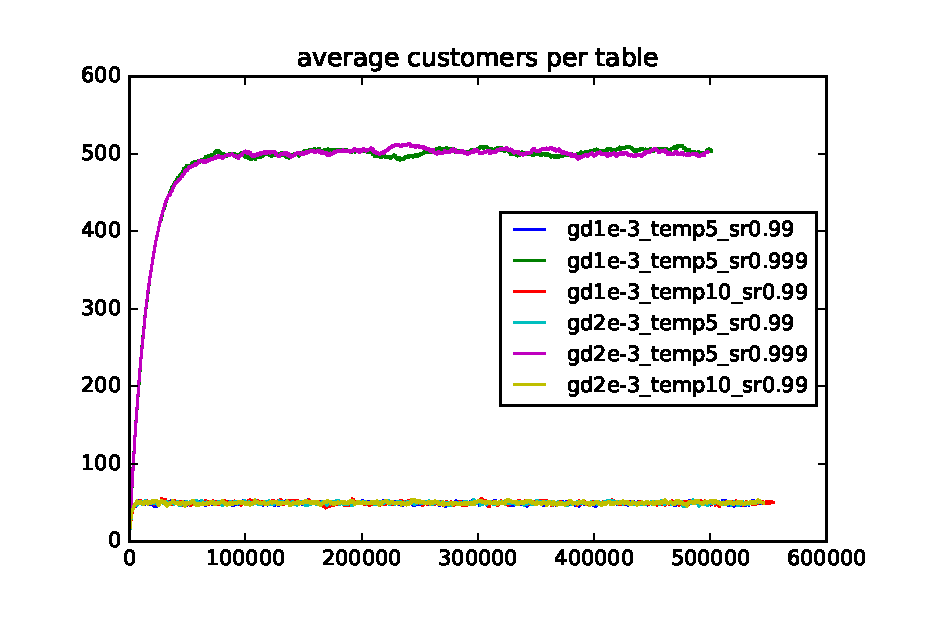
\includegraphics[width = \textwidth]{plans/eps/0_1_2_3_4_5_cnum_avg.eps}
    \caption{}
    \label{fig::plans_a}
  \end{subfigure}
  \begin{subfigure}{0.49\textwidth}
    \centering
    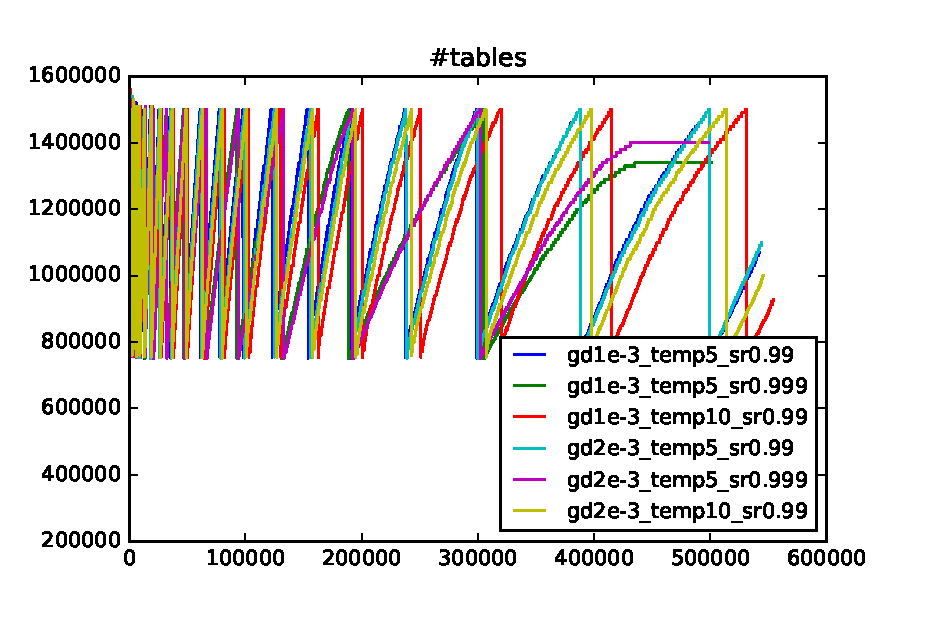
\includegraphics[width = \textwidth]{plans/eps/0_1_2_3_4_5_rest_num.eps}
    \caption{}
    \label{fig::plans_b}
  \end{subfigure}
  \\
  \begin{subfigure}{0.49\textwidth}
    \centering
    \includegraphics[width = \textwidth]{plans/eps/0_1_2_3_4_5_reduce_cnt.eps}
    \caption{}
    \label{fig::plans_c}
  \end{subfigure}
  \begin{subfigure}{0.49\textwidth}
    \centering
    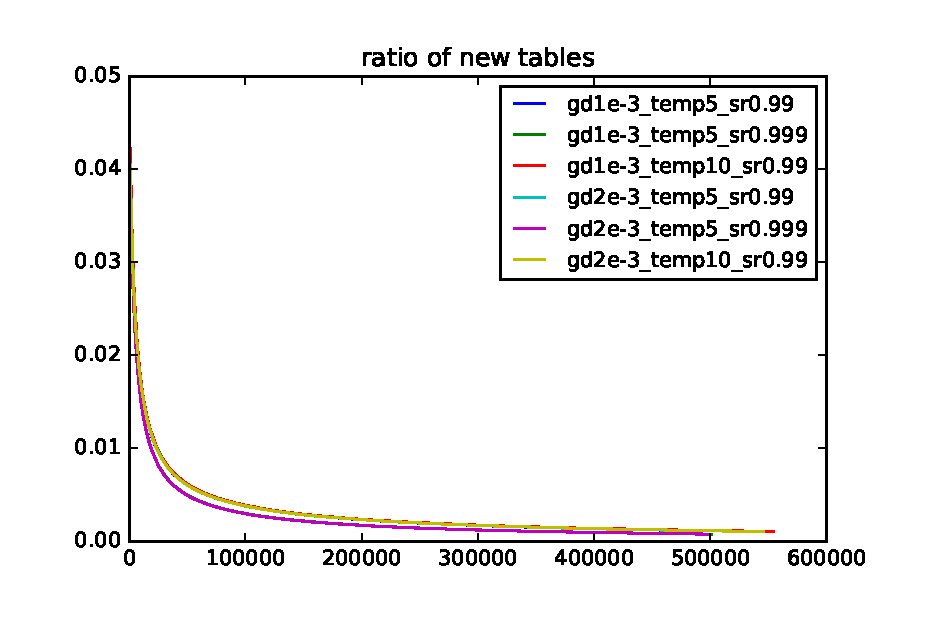
\includegraphics[width = \textwidth]{plans/eps/0_1_2_3_4_5_miss.eps}
    \caption{}
    \label{fig::plans_d}
  \end{subfigure}
  \caption{Curves of average customers per table, number of tables, the number
    of days when tables are pruned, and ratio of customers being assigned to a new
  table. The x-axis is the total number of customers so far. }
  \label{fig::plans}
\end{figure}

To this end, we specifically plot the curves of average customers per table, the
number of tables, the number of days when tables are pruned, and the ratio
between the number of customers being assigned to a new table and all customers.
In Figure~\ref{fig::plans}, the X-axis is the number of customers entering the
restaurant so far. With 48 threads, it was found that appropriate gradient
descent step size ranges from \SI{5e-4} to \SI{4e-3}. Useful final temperature
is from $0.1$ to $0.5$ and the shrink rate $\beta$ from $0.95$ to $0.999$.

Note that the in the curve \ref{fig::plans_a}, $\beta$ is the most influencing
factor. With a larger $\beta = 0.999$, fewer customers are leaving the restaurant
per day. This also contributes to the fact that the tCRP will explore fewer new
tables than with a smaller $\beta = 0.99$, as seen in Figure~\ref{fig::plans_d};
we see a smaller ratio of customers is assigned to new tables. In addition, from
Figure~\ref{fig::plans_c}, we observe that both a larger $\beta$ or a smaller
final temperature can yield fewer number of table pruning. To see this,  note
that with a small final temperature, the stochasticity of PLANS is reduced
exponentially.

\subsection{Classification Experiment}

In this part, we will use the learnt embedding of phrase to represent documents
and see if that can benefit text classification. It was previously shown that by
combining low-dimensional embedding with bag-of-words representation, the
performance can be improved.

We use a classic sentiment classification dataset~\cite{pang2002thumbs}, which
has a set of 700 positive and 700 negative processed movie reviews collected
from the IMDB archive. The dataset is tokenized and words are normalized
already. We followed the use of the data by dividing it into three equal-sized
folds, maintaining balanced class distribution in each fold.  All results
reported below are the average of three-fold cross-validation evaluation on the
dataset.  We use the Logistic-Regression in Scikit-Learn
package~\cite{scikit-learn} for the binary (positive/negative) polarity
classification with different representation strategies for the review
documents.

\begin{table}[h]
  \centering
  \begin{tabular}{c|c|c|c|c|c}
    & Sparse Features & Sparse Dim & Dense Features & Dense Dim & Accuracy \\
    \hline \hline
    (1) & Unigram     & 31,240 & \emph{N.A}  & 0   & 67.512 \\
    (2) & \emph{N.A}  & 0      & Word        & 100 & 58.471 \\
    (3) & \emph{N.A}  & 0      & Phrase      & 100 & 60.332 \\
    (4) & Unigram     & 31,240 & Word        & 100 & 73.637 \\
    (5) & Unigram     & 31,240 & Phrase      & 100 & 77.952 \\ \hline \hline
  \end{tabular}
  \caption{Average three-fold cross-validation accuracies, in percent.}
  \label{tab::plans_cls}
\end{table}

In the experiment, we find $31,240$ unique terms in the reviews. However, note
not all of those words are the top 0.1M frequent words in the NY Times corpus
and it might not always true that there is an embedding vector for each word in
the reviews. From the above Table~\ref{tab::plans_cls}, we see that with the
sparse feature (unigram) only, the baseline performance is merely $67.512\%$.
The unigram baseline is better than only using dense embedding as features.  We
offer two reasons to explain this result: 1) Some discriminative words for
sentiment polarity in the dataset might not has an embedding learnt from the NY
Times and therefore information of those words is lost in the embedding
representation; and 2) The dimension of dense embeddings is only 100 while the
sparse feature has a dimension of $31,240$. Thus models learnt with only dense
embeddings is limited in its capacity to fit the training data and it is
expected that the performance is worse than (1). Comparing (2) and (3), it is
seen that with phrase embeddings learnt from PLANS, there is still a marginal
improvement in performance.

Nevertheless, when combining sparse unigram and dense embedding together, we
observe the best performances. The accuracy for ``unigram+word'' (4) is $73.637$
while the accuracy reaches $77.952$ for ``unigram+phrase'' (5). It is clear that
phrase embeddings learnt by PLANS significantly boost the performance for
polarity classification than that of word embedding. This is also consistent
with the finding by \cite{pang2002thumbs} that bigrams can also benefit the
sentiment classification.

